\chapter{Greenhouse Software}
\label{chap:appendix}
%Reducing the spacing from the title


Here you write the context of the appendix, structuring such content in
sections, sub-sections and sub-sub-sections, if needed.

An example of appendix is the flat presentation of all the graphical user interface screens.
Each screen can be presented (identification symbol and description) and screens transition graph can be given.


\section{Login}
\label{sec:appendix_Login}
\begin{figure}
\includegraphics[width=1\textwidth]{images/mockup_login_eps.eps}
\end{figure}

The 'Login' page is the first page everyone sees before being able to use any
features of our software.

The User needs to identify himself with valid credentials.

\subsection{Username}
This input field is used for the \emph{Username} of the Gardener, Technician or
Manager.

\subsection{Password}
This input field is used for the \emph{Password} of the Gardener, Technician, or
Manager.

\subsection{Sign In Button}
This button send the request to be signed in, by clicking it.

\subsubsection{Success Scenario}
The \emph{User} is taken the \emph{Home} screen.

\subsubsection{Failure Scenario}
The \emph{User} gets a visible error message.





\section{Home}
\label{sec:appendix_Home}
\begin{figure}
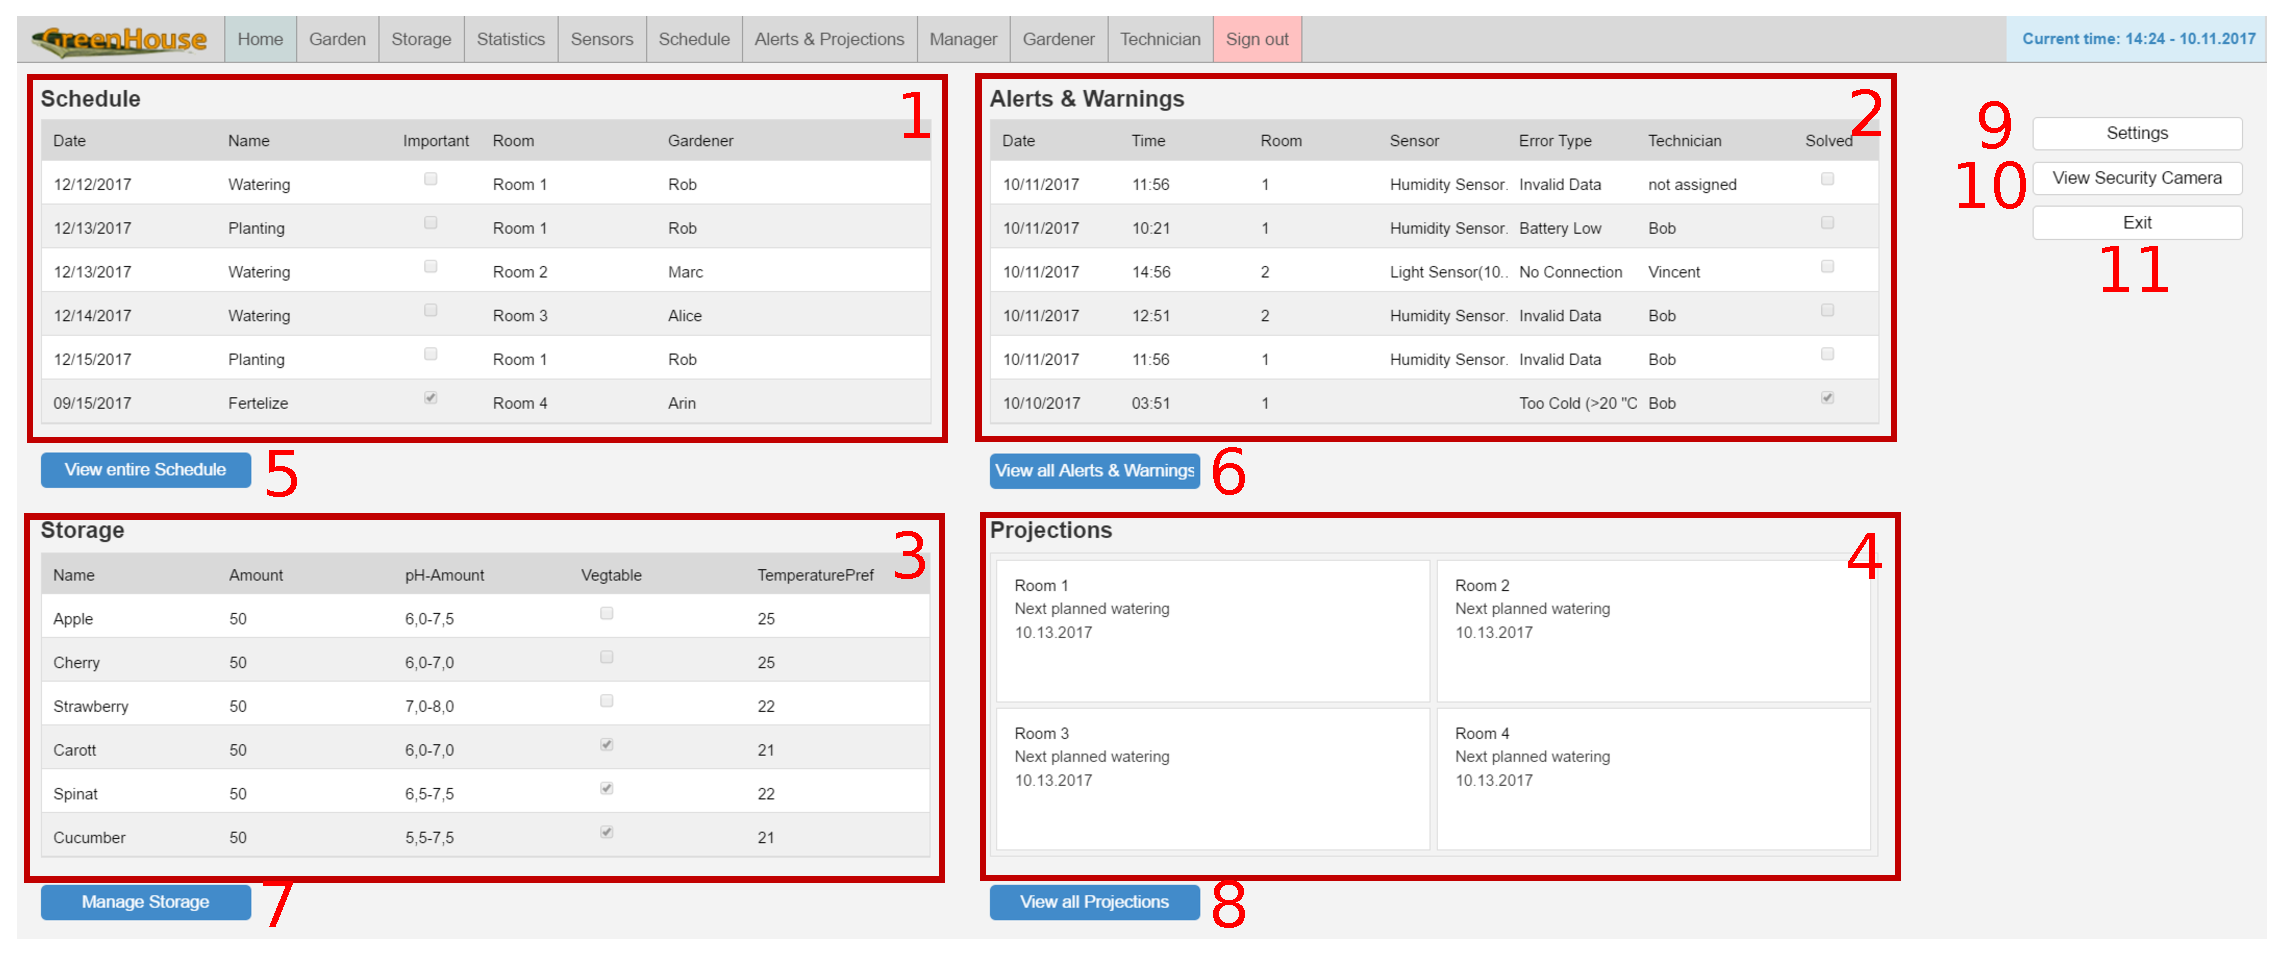
\includegraphics[width=1\textwidth]{images/mockup_home_eps.eps}
\end{figure}

The \emph{Home} page is the first page the \emph{User} sees after signing in.

This page gives a quick summary of the most important information about the most
recent alerts and warning, the next upcoming tasks and planned watering for each
room and low running stock. 

Further accesses through the blue and white buttons.

\subsection{Schedule}
The \emph{Schedule} shows a summary of the 6 next upcoming tasks of the
gardeners. The list contains information about the \emph{Date}, the \emph{Task
name}, the concerned \emph{Room} and \emph{Gardener} and a checkbox indicating
whether the task is \emph{Important}.

\subsection{Alerts and Warnings}
The \emph{Alerts and Warnings} list shows a summary of the 6 latest Alerts and
Warnings for the \emph{Technician}. The list contains information about the
\emph{Date} and \emph{Time} the alert or warning was added to the system, the
concerned \emph{Room} and \emph{Sensor} if there is a sensor assigned to the
alert or warning. The \emph{Error Type} gives more precise information about the
malfunctioning if it an alert. For Warnings is describes the Problem.
Additionally we get Information about the assigned \emph{Technician} if assigned
and if the problem is already \emph{Solved}.

\subsection{Storage}
The \emph{Storage} list shows a summary of the 6 items with the lowest quantity.
The list contains information about the \emph{Name} of the items, the current
\emph{Amount}. The other information about the \emph{pH-Amount, Vegetable and
TemperaturePref} are used to distinguish between more types of the same plant.

\subsection{Projections}
The \emph{Projections} grid shows a summary of the 4 next rooms planned
to be watered. The single grid contains informations about the concerned
\emph{Room} and the \emph{Date} for the next planned watering.

\subsection{View entire Schedule Button}
The \emph{View entire Schedule} button is a shortcut from the menu
\emph{Schedule} button. The button is designed for a fast access and has a blue
color.

\subsection{View all Alerst and Warnings Button}
The \emph{View all Alerts and Warnings} button is a shortcut from the menu
\emph{Alerts and Projections} button. The button is designed for a fast access
and has a blue color.

\subsection{Manage Storage Button}
The \emph{Manage Storage} button is a shortcut from the menu
\emph{Manager} button. The button is designed for a fast access and has a blue
color.

\subsection{View all Projections Button}
The \emph{View all Projections} button is a shortcut from the menu
\emph{Alerts and Projections} button. The button is designed for a fast access
and has a blue color.

\subsection{Settings Button}
The \emph{Settings} button opens a pop-up window with the \emph{Settings}
screen.

\subsection{View Security Camera Button}
The \emph{View Security Camera} button opens a pop-up window with the
\emph{Security Camera} screen.

\subsection{Exit Button}
The \emph{Exit} button signs the current \emph{User} out and closes the
\emph{Greenhouse} Software application.

